\documentclass{article}
\usepackage[magyar]{babel}
\usepackage{t1enc}
\usepackage{graphicx}
\usepackage{amsmath}
\usepackage[export]{adjustbox}
\usepackage{siunitx}
\graphicspath{ {./images/} }

\title{Ohm és Kirchhoff törvényei}
\author{Bejó Dávid}
\date{2024}

\begin{document}

\maketitle

\section{Bevezetés}
Az Ohm-törvény és a Kirchhoff-törvények az elektrotechnika és a fizika területén alapvető elvek, amelyek alapvető keretet biztosítanak az elektromos áramkörök megértéséhez és elemzéséhez. Ezek a törvények képezik az áramkörelmélet sarokkövét, lehetővé téve a mérnökök és a tudósok számára az elektromos rendszerek előrejelzését, tervezését és hibaelhárítását.

\section{Ohm törvénye}
Ha két változó mennyiség hányadosa állandó, akkor azt mondjuk, hogy a két mennyiség egyenesen arányos. A fogyasztóra kapcsolt feszültség egyenesen arányos a fogyasztón átfolyó áram erősségével. \cite{ohm} Ez Ohm törvénye. Nevét felfedezőjéről, Georg Simon Ohm (1787–1854) német fizikusról kapta. Róla nevezték el az elektromos ellenállás mértékegységét. Ohm törvényének alapegyenlete a következő:
\begin{equation}
    U = I \cdot R
\end{equation}
ahol:
\begin{itemize}
    \item $U$ a fogyasztón mért feszültséget jelenti voltban (V),
    \item $I$ a fogyasztón átfolyó áram amperben kifejezve (A),
    \item $R$ a fogyasztó ellenállása ohmban ($\Omega$).
\end{itemize}

\section{Feszültség, áramerősség és ellenállás}
\subsection{Feszültség (\textit{V})}
A feszültség megmutatja, hogy mennyi munkát végez az elektromos mező, miközben 1 C töltést a mező egyik pontjából a másikba áramoltat.

\subsection{Áramerősség (\textit{I})}
Az áramerősség megmutatja, hogy mekkora a vezető keresztmetszetén 1 s alatt átáramlott elektromos tulajdonságú részecskék együttes töltése.

\subsection{Ellenállás (\textit{R})}
A fogyasztóknak azt a tulajdonságát, hogy anyaguk részecskéi akadályozzák az elektromos tulajdonságú részecskék áramlását.

\section{Ohm törvénye soros és párhuzamos kapcsolásokban}

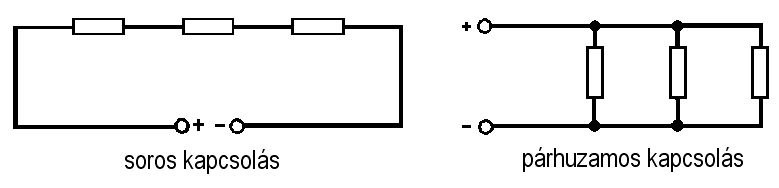
\includegraphics[width=\textwidth]{kapcsolasok}

\subsection{Soros kapcsolás}
Ha két ellenállásnak csak az egyik vége van összekötve, és közéjük semmi más nem kapcsolódik, akkor a két elem sorba van kapcsolva. A sorosan kapcsolt ellenállások összege egyenlő az eredő ellenállás ($R_{\text{eredő}}$) összegével:
\begin{equation}
    R_{\text{eredő}} = R_1 + R_2 + \ldots + R_n
\end{equation}

\subsection{Párhuzamos kapcsolás}
Párhuzamos kapcsolásnak azt nevezzük, amikor az alkatrészek azonos végüknél vannak összekötve.
Az eredő ellenállás reciproka egyenlő a párhuzamosan kapcsolt ellenállások reciprokainak összegével:
\begin{equation}
    \frac{1}{R_{\text{eredő}}} = \frac{1}{R_1} + \frac{1}{R_2} + \ldots + \frac{1}{R_n}
\end{equation}
\pagebreak
\section{Kirchhoff-törvények}
A Kirchhoff-törvények a villamosságtanban a töltés és az energia megmaradását tárgyalják. Először Gustav Kirchhoff (1824-1887) mondta ki őket 1845-ben. 

\section{Kirchhoff I. törvénye: a csomóponti törvény}
Kirchhoff csomóponti törvénye szerint a csomópontba befolyó áramok összege megyegyezik a csomópontból kifolyó áramok összegével, azaz a csomópont áramainak előjelhelyes összege nulla. \cite{kirchhoff1}

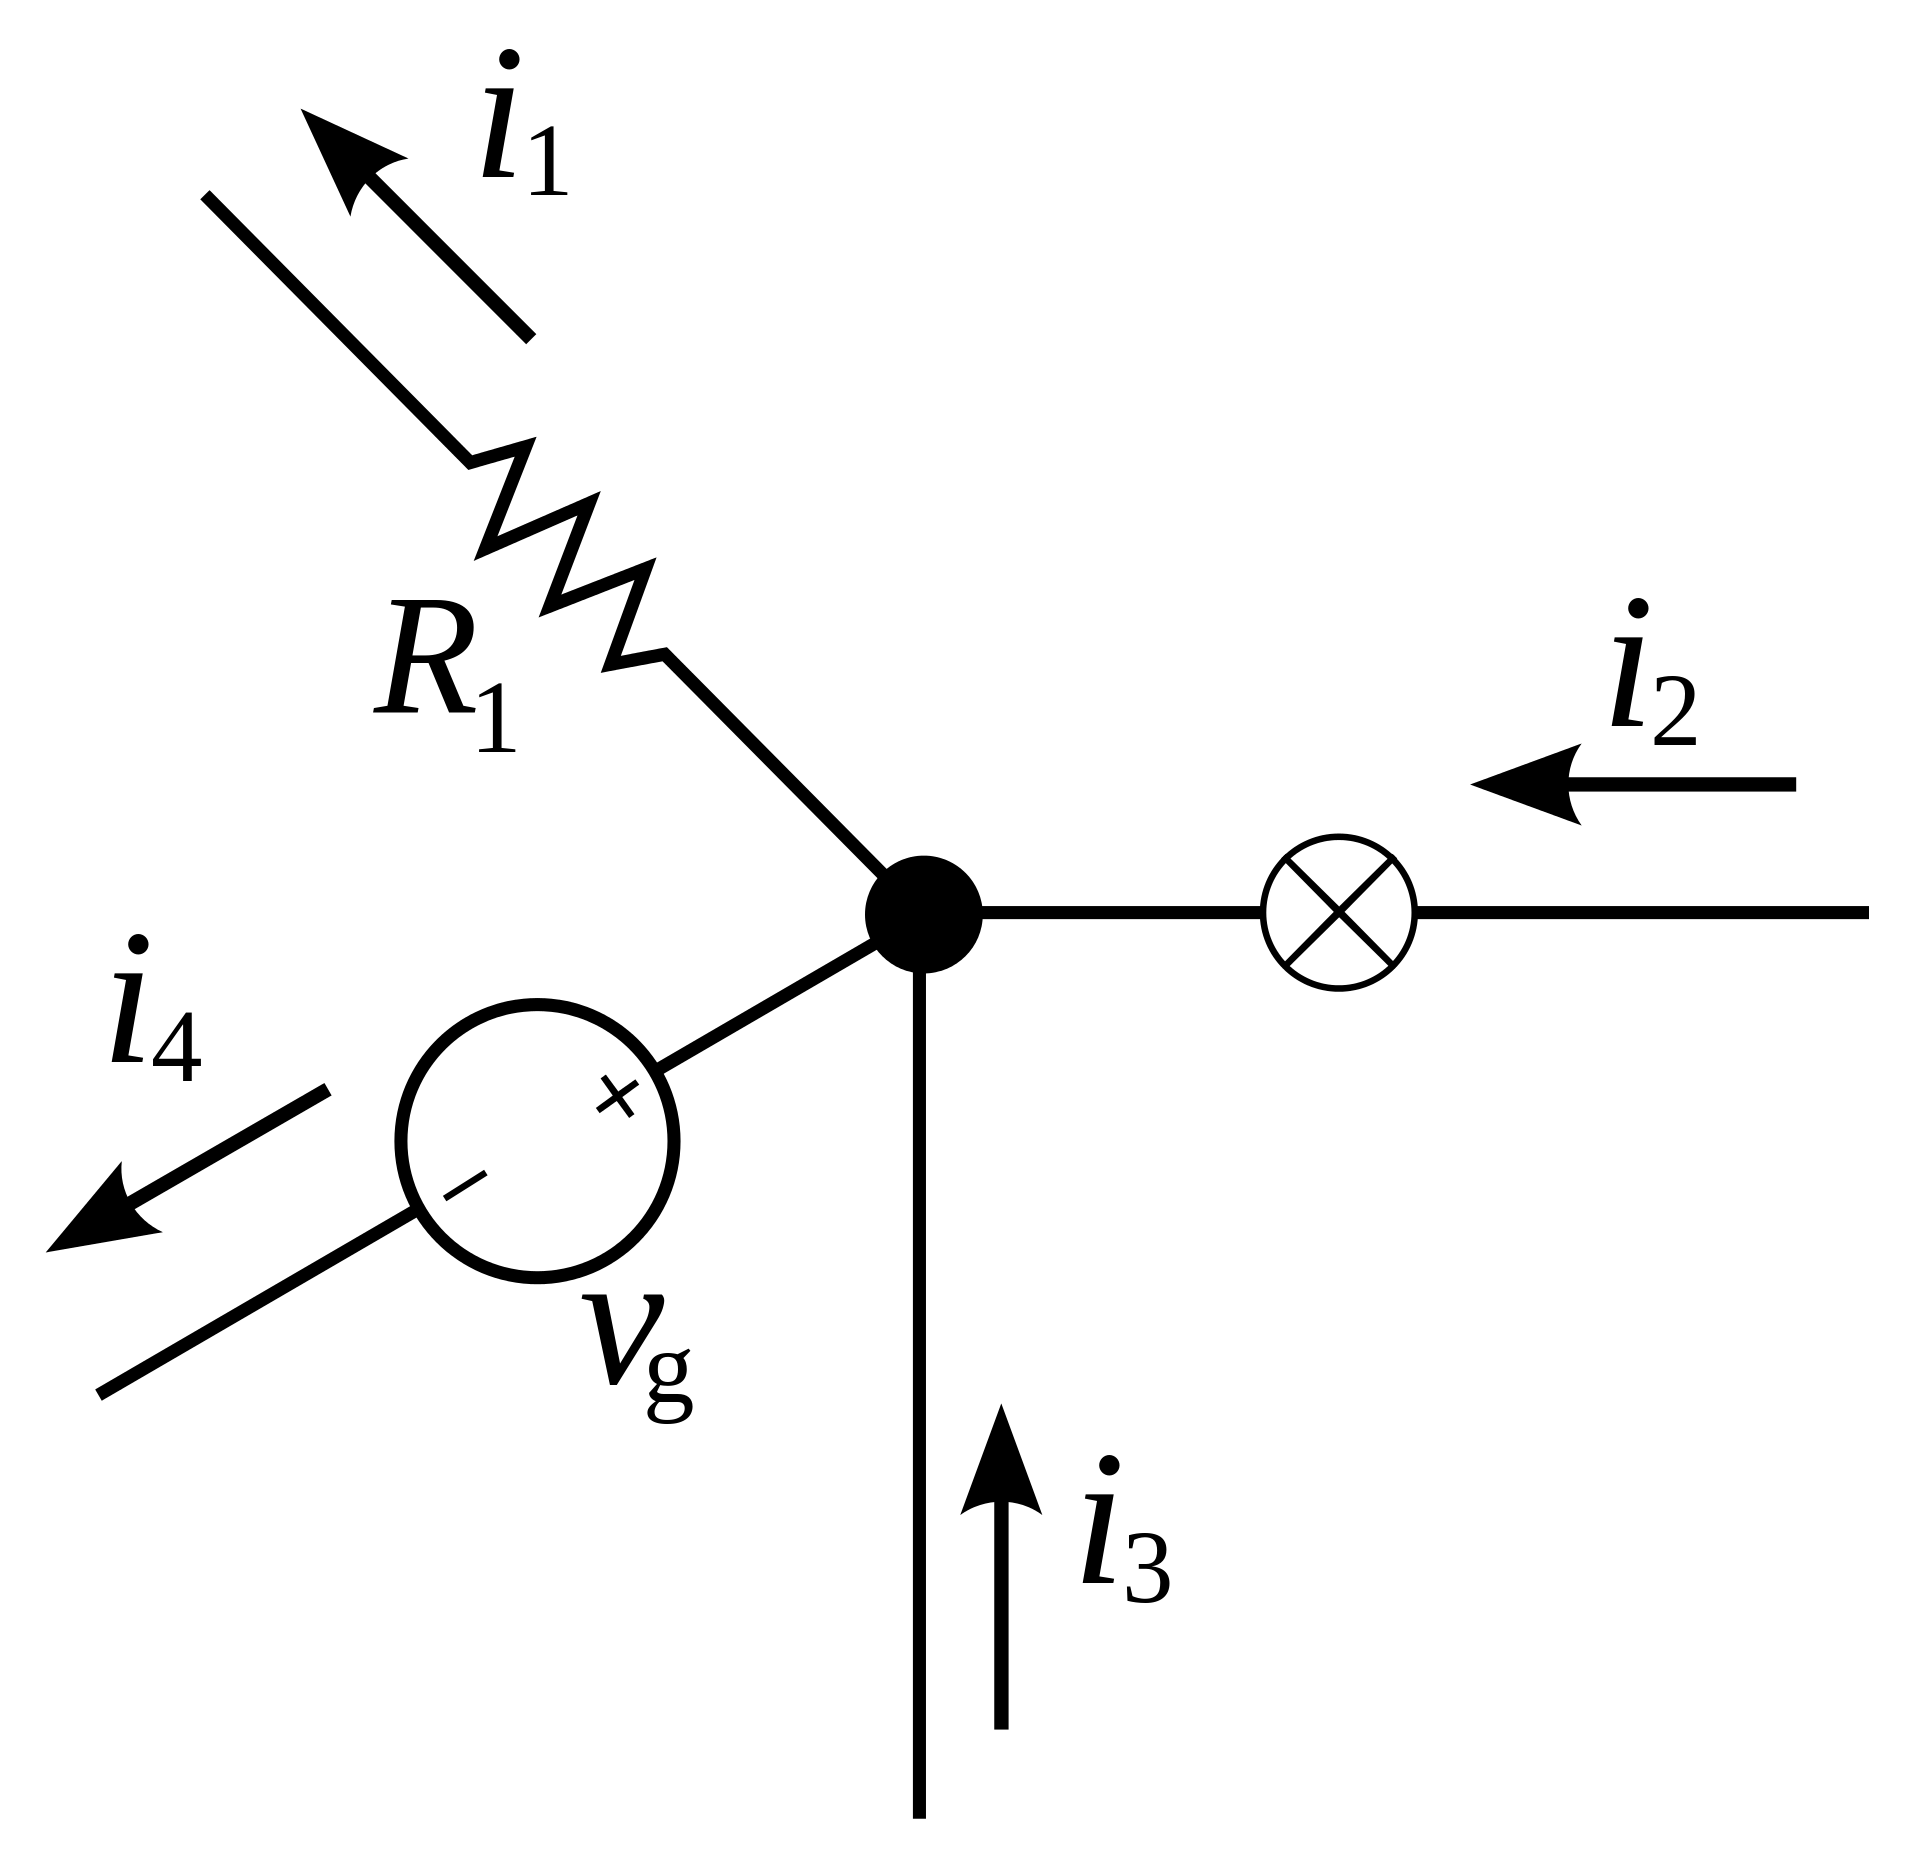
\includegraphics[width=5cm, center]{kirchoff1}

Matematikai képlettel kifejezve:
\begin{equation}
    \sum_{n} I_n = 0
\end{equation}

\section{Kirchhoff II. törvénye: a huroktörvény}
A törvény értelmében bármely zárt hurokban a feszültségek előjeles összege nulla. \cite{kirchhoff2)

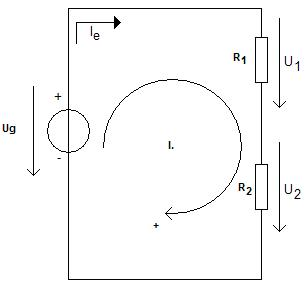
\includegraphics[width=5cm, center]{kirchoff2}

Matematikai képlettel kifejezve:
\begin{equation}
    \sum_{n} U_n = 0
\end{equation}

\section{Kirchhoff-törvények alkalmazása}
A fentebb ismertetett három törvény: az Ohm törvény, valamint Kirchhoff I. és II. törvénye a villamos hálózatokkal kapcsolatos számítások három alaptörvénye. Ezek a törvények biztosítják a szükséges eszközöket az elektromos áramkörök összetett viselkedésének elemzéséhez és megértéséhez. Alkalmazásuk széles körű, beleértve az áramköri tervezést, hibaelhárítást és az elektronikai eszközök fejlesztését is.

\section{Áramosztó kapcsolás}
Az áramosztó kapcsolás egy olyan elektromos áramkör, ahol az áram az egyik ágban megoszlik több ág között. Ez a kapcsolás gyakran alkalmazott áramkörökben, ahol különböző áramokat vagy terheléseket kell táplálni.

\subsection{Áramosztó kapcsolások elve}
Az áramosztó kapcsolásban a főáram ág (melynek ellenállása $R_s$) elágazik több mellékágra ($R_1$, $R_2$, stb.), amelyek párhuzamosan vannak kapcsolva. Az árammegoszlás az ágak ellenállásaik arányában történik.

\subsection{Áramosztó kapcsolások számítása}
Az áramokat a főágon és a mellékágakon az Ohm-törvény alapján lehet számolni. Az áramok arányát a főágon és az egyes mellékágakon az ellenállások arányával kaphatjuk meg.

\subsection{Áramosztó kapcsolás példa}
Az áramosztó főága $R_s$ ellenállással rendelkezik, míg a két mellékág $R_1$ és $R_2$ ellenállásokkal. Az áramokat a főágon ($I_s$) és a mellékágakon ($I_1$, $I_2$) az alábbi módon számolhatjuk:
\begin{align*}
I_s &= \frac{U}{R_s} \
I_1 &= \frac{U}{R_1} \
I_2 &= \frac{U}{R_2}
\end{align*}

A következő táblázat bemutatja az áramosztó kapcsolás példáját különböző $R_1$ és $R_2$ értékek mellett. A forrási áramerősség konstans értéke $I_s = 10$ A.

\begin{center}
\begin{tabular}{|c|c|c|}
\hline
\textbf{$R_1$ (\si{\ohm})} & \textbf{$R_2$ (\si{\ohm})} & \textbf{$I_1$ (\si{\ampere})} \\
\hline
100 & 100 & 5 \\
200 & 100 & 6.67 \\
300 & 100 & 7.5 \\
\hline
\end{tabular}
\end{center}

Az $I_1$ értékek azt mutatják, hogy hogyan változik az első ágon mért áramerősség az $R_1$ és $R_2$ értékek függvényében. Ahogy látható, az $I_1$ érték növekszik az $R_1$ növekedésével és az $R_2$ csökkenésével.

Ez a táblázat segíthet abban, hogy jobban megértsük az áramosztó kapcsolás működését és annak hatását az ágakban mért áramerősségekre különböző ellenállásértékek mellett.

\section{Feszültségosztó kapcsolás}
A feszültségosztó kapcsolás egy olyan elektromos áramkör, ahol a feszültség megoszlik több ág között, amelyek párhuzamosan vannak kapcsolva. Ez a kapcsolás gyakran alkalmazott áramkörökben, ahol különböző feszültségekre van szükség.

\subsection{Feszültségosztó kapcsolások elve}
A feszültségosztó kapcsolásban a forrási feszültség (amelynek értéke $U_s$) eloszlik a különböző ágakon úgy, hogy az arányuk megegyezik az ágak ellenállásainak arányával.

\subsection{Feszültségosztó kapcsolások számítása}
A feszültségeket az egyes ágakon az Ohm-törvény és a feszültségosztó elve alapján lehet kiszámolni.

\subsection{Feszültségosztó kapcsolás példa}
Az ágak ellenállásai $R_1$ és $R_2$. A feszültségeket az egyes ágakon ($U_1$ és $U_2$) az alábbi módon számolhatjuk:
\begin{align*}
U_1 &= U_s \cdot \frac{R_1}{R_1 + R_2} \
U_2 &= U_s \cdot \frac{R_2}{R_1 + R_2}
\end{align*}

A következő táblázat bemutatja a feszültségosztó kapcsolás példáját különböző $R_1$ és $R_2$ értékek mellett. A forrási feszültség konstans értéke $U_s = 10$ V.

\begin{center}
\begin{tabular}{|c|c|c|}
\hline
\textbf{$R_1$ (\si{\ohm})} & \textbf{$R_2$ (\si{\ohm})} & \textbf{$U_1$ (\si{\volt})} \\
\hline
100 & 100 & 5 \\
200 & 100 & 6.67 \\
300 & 100 & 7.5 \\
\hline
\end{tabular}
\end{center}

Az $U_1$ értékek azt mutatják, hogy hogyan változik az első ágon mért feszültség az $R_1$ és $R_2$ értékek függvényében. Ahogy látható, az $U_1$ érték növekszik az $R_1$ növekedésével és az $R_2$ csökkenésével.

Ez a táblázat segíthet abban, hogy jobban megértsük a feszültségosztó kapcsolás működését és annak hatását az ágakban mért feszültségekre különböző ellenállásértékek mellett.

\begin{thebibliography}{2}
\bibitem{ohm} Georg Simon Ohm: \textit{Die galvanische Kette, mathematisch bearbeitet}
\bibitem{kirchhoff1} Gustav Robert Kirchhoff: \textit{Vorlesungen über mathematischen Physik: Mechanik}
\bibitem{kirchhoff2} Gustav Robert Kirchhoff: \textit{Vorlesungen über mathematischen Physik: Elektricitätslehre}
\end{thebibliography}


\end{document}
